\section{Grundlagen}
Im Grundlagenkapitel stellen Sie das Basiswissen für die weiteren Kapitel vor. Hierzu können neben theoretischen Konzepten auch die historische Entwicklung und aktuelle Forschungsvorhaben gehören. Idealerweise bedient man sich hier mehrerer verschiedener Quellen, um die Ausführungen zu belegen.

Nachfolgend werden einige Formalitäten der Arbeit dargestellt.

Zur korrekten Verwendung der Vorlage benötigen Sie die TU Darmstadt Schriftart: \href{https://www.tu-darm-stadt.de/kommunikation_und_medien/corporate_design_1/schriften_und_vorlagen/index.en.jsp}{Schriften und Vorlagen der TU Darmstadt}
\subsection{Gliederungen}
Text
\subsubsection{Gliederungsebene 3}
Text
\paragraph{Gliederungsebene 4}
Text
\subsection{Aufzählungen}
\begin{itemize}
	\item Fehlende Motivation,
	\item Fehlende Agilität und 
	\item Fehlende Compliance.
\end{itemize}

Text 
\newpage
\subsection{Abbildungen}

\begin{figure}[h]
\begin{center}

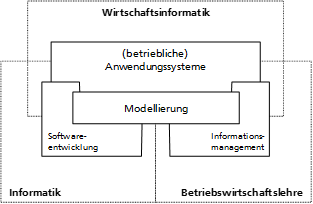
\includegraphics[width=10cm]{images/Abb2_3.png}
\caption{Einordnung der Wirtschaftsinformatik (angelehnt an Fink et al. 2001)}
\label{Abbildung2_3}
\end{center}
\end{figure}
Bitte achten Sie darauf, dass alle vorhandenen Abbildungen und Tabellen in einem inhaltlichen Zusammenhang mit dem Text stehen und Sie auf die entsprechende Abbildung (bspw. Abbildung 1) verweisen.
\subsection{Tabellen}
%hier Tabelle einfügen
\begin{table}[h]
\centering
\begin{tabular}{ccc}
\hline \textbf{Attribute} &\textbf{Typ}  & \textbf{1. Ausprägung (Beispiel)} \\ 
\hline Titel & \textit{STRING}& Aktiengesetz (AktG)  \\ 
Text& \textit{STRING} &  [Text des AktG]\\ 
Gültig von & \textit{DATE} & 01.01.2010 \\ 
Gültig bis & \textit{DATE} & - \\ 
Dok.-Besitzer & \textit{STRING} & Rechtsabteilung \\ 
Quelle & \textit{STRING}  & Deutsche Gesetze \\ 
Verplichtungsgrad & \textit{STRING} & verplichtend \\ 
\hline 
\end{tabular} 
\caption{Attribute der Anforderungsquellen im Metamodell}
\label{tab:tabelle 1}
\end{table}
\par\medskip

Tabelle 1 stellt eine beispielhafte Tabelle dar